\chapter{Einleitung}
\section{Allgemeines}
Ein Audio-Bluetooth-Modul soll in einfacher Weise ein Audio-Signal von beispielsweise einem Smartphone ausgeben. Dabei ist eine hohe Kompatibilität mit viele Geräten wichtig, weil es sehr viele verschiedene Versionen von Bluetooth gibt. Da Bluetooth-Geräte meist abwärtskompatibel sind, ist es sinnvoll das Modul mit einer älteren BT-Version laufen zu lassen.

\section{Zielsetzung}
Es soll ein Print angefertigt werden auf dem sich das BT-Modul samt Versorgungsschaltung befindet. Auf diesem Print wird zusätzlich noch eine Additionsschaltung vorgesehen, um auch mit einem Klinkeneingang ein Signal zuführen zu können, falls das BT-Modul ausfällt.\\
Um eine leichtere Handhabung zu ermöglichen, muss auch ein Adapterprint für das BT-Modul angefertigt werden.

\section{Auswahl des Bluetooth-Moduls}
Wie bereits erwähnt soll das BT-Modul mit möglichst viele Geräten kompatibel sein, also mit einer älteren BT-Version laufen. Es sollte weiterhin eine möglichst einfache Bedienung für den Benutzer ermöglichen (beispielsweise Play-/Pausetaste).\\
Außerdem soll es bei geringen Kosten eine möglichst gute Verbindung, d.h. einen hohe Reichweite, erzielt werden.\\ \\
Nach ausführlicher Recherche wurde das Modul \enquote{XS3868 Revision 3} ausgewählt. Der darauf verbaute Chip \enquote{OVC3860} von \enquote{OmniVision Technologies} hat sich bereits in vielen anderen Projekten bewährt. 

\chapter{Bluetooth-Modul XS3868}
\section{OVC3860}
In dem Chip ist außer der Bluetooth-Verbindung auch noch ein Stereo-Audio-Prozessor verbaut. Zusätzlich gibt es noch eine UART-Schnittstelle mithilfe man einige Einstellungen am Chip vornehmen kann. Eine kleine LiPo-Ladeschaltung ist ebenfalls vorhanden, wird aber in diesem Fall nicht verwendet.\\
Das Modul benötigt eine Versorgungsspannung von 3,3V bis 4,2V, wobei der Chip mit 1,8V versorgt wird. Diese Spannung wird auf dem Modul erzeugt.\\
Die verwendete BT-Version ist 2.0. Einige GPIO-Pins sind auf das Modul herausgeführt um Funktionen wie \enquote{Play/Pause} zu ermöglichen. Der Chip benötigt einen externen Speicher um ordnungsgemäß zu funktionieren.
\begin{figure} [h]
	\centering
	\caption{Blockschaltbild OVC3860}
	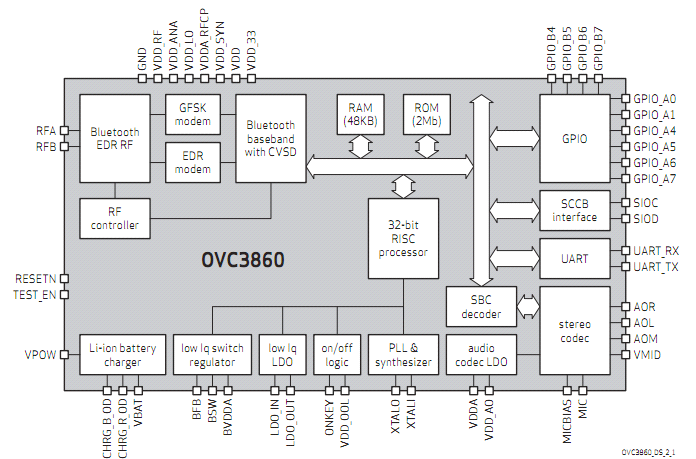
\includegraphics[width=0.8\textwidth]{img/blockschaltbild.png}
\end{figure}

\section{Pinbelegung}
Insgesamt hat das Modul 23 verwendbare Pins, aufgeteilt auf 2 Seiten in 11 und 12 Pins. 
\begin{figure} [h]
	\centering
	\caption{Pinbelegung XS3868}
	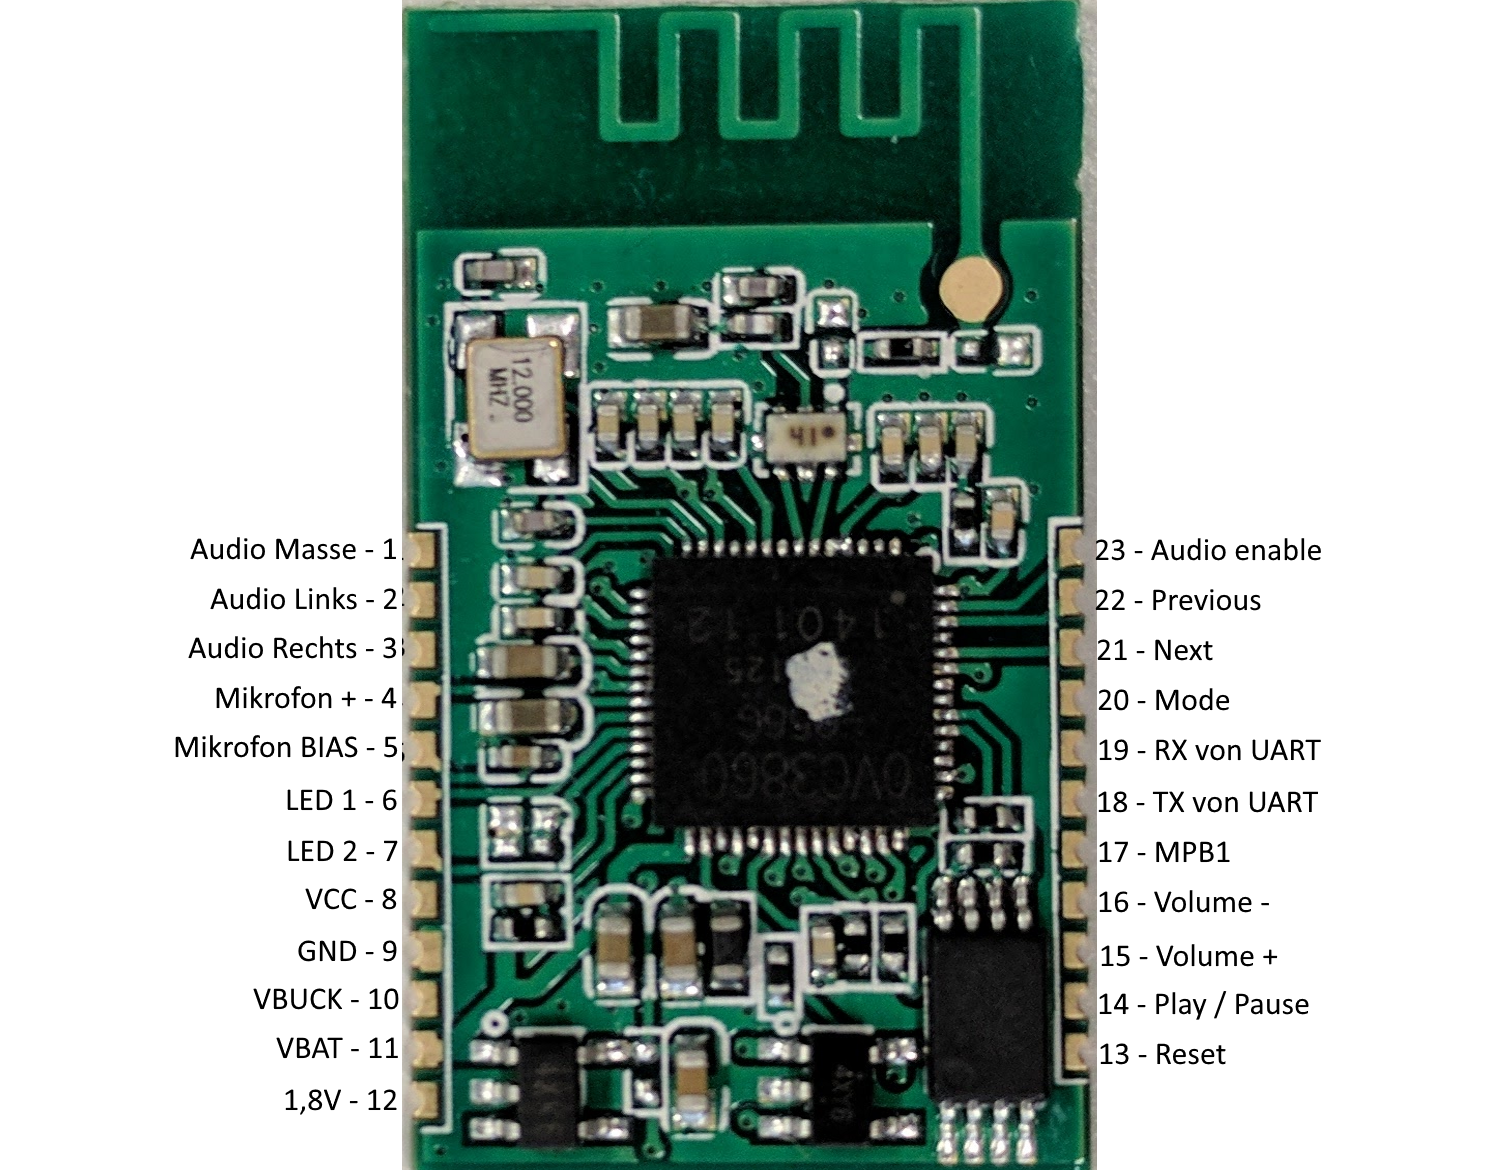
\includegraphics[width=1\textwidth]{img/XS3868_Pinbelegung.png}
\end{figure}

